\section{Findings}
\label{sec:findings}

We organize the findings around the three research questions. Section~\ref{sec:encounters} examines how participants read the Trashbots through their interactions and post-encounter accounts (\textbf{RQ1}). Section~\ref{sec:process} examines the strategies participants used to make sense of the robots' presence (\textbf{RQ2}). Section~\ref{sec:site-sensemaking} examines the factors that influenced how participants read the robots' actions and whether those factors were specific to the encounter site (\textbf{RQ3}). The comparative analysis includes 86 interview records from Tappen Park, Astoria Park, Little Italy, Campus Caf\'e, and Navy Yard. Participants are identified by site and interview number: TP for Tappen Park, AP for Astoria Park, LI for Little Italy, CC for Campus Caf\'e, and NY for Navy Yard.

\subsection{Encountering the Trashbot: Interactions, First Impressions, and Perceived Roles}
\label{sec:encounters}

To address \textbf{RQ1}, we examined how participants read the the Trashbots through observable interaction and through their post-encounter accounts of attitude, first impressions, and perceived roles. Figure~\ref{fig:rq1-pooled-codes} summarizes the prevalence of the interview codes across the 86 records, while Table~\ref{tab:codes-by-site-5-1} compares the same codes across deployment sites. Impression and perceived-role codes could co-occur within an interview record.

Encounters with the Trashbot were generally brief and opportunistic. People deposited waste when the robot came within reach, approached after watching how it moved, waved toward its camera, photographed or recorded it, or observed it from a distance. Figure~\ref{fig:site-encounters} shows examples from five deployment sites, one in each borough. At the campus caf\'e, CC-P04 recalled, \emph{``I didn't know what it was at first''}; nonetheless, he got up with an empty coffee cup and \emph{``slowly walked towards it.''} This account shows that interaction could begin while the robot's purpose was still uncertain.

\begin{figure*}[ht]
  \centering
  \begin{subfigure}[t]{0.30\textwidth}
    \centering
    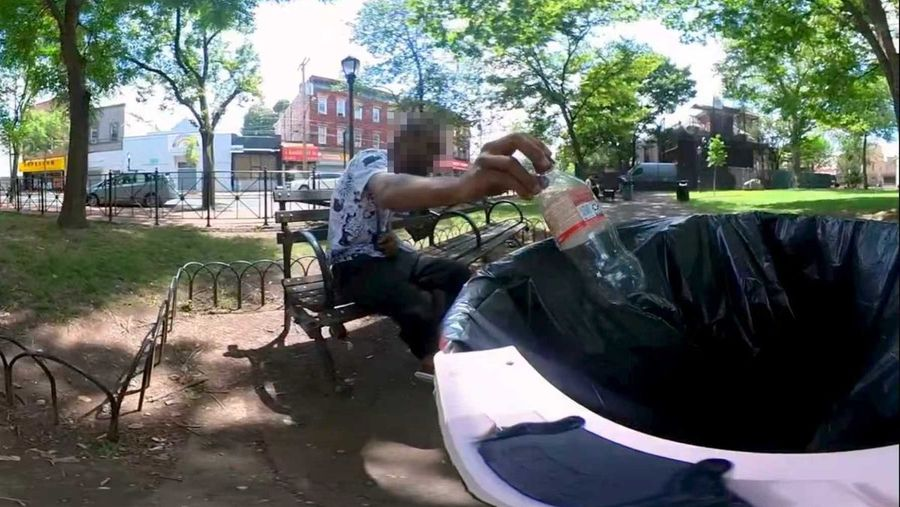
\includegraphics[width=\linewidth]{figures/vignettes/c_tappen_bottle.jpg}
    \caption{Tappen Park}
  \end{subfigure}\hfill
  \begin{subfigure}[t]{0.30\textwidth}
    \centering
    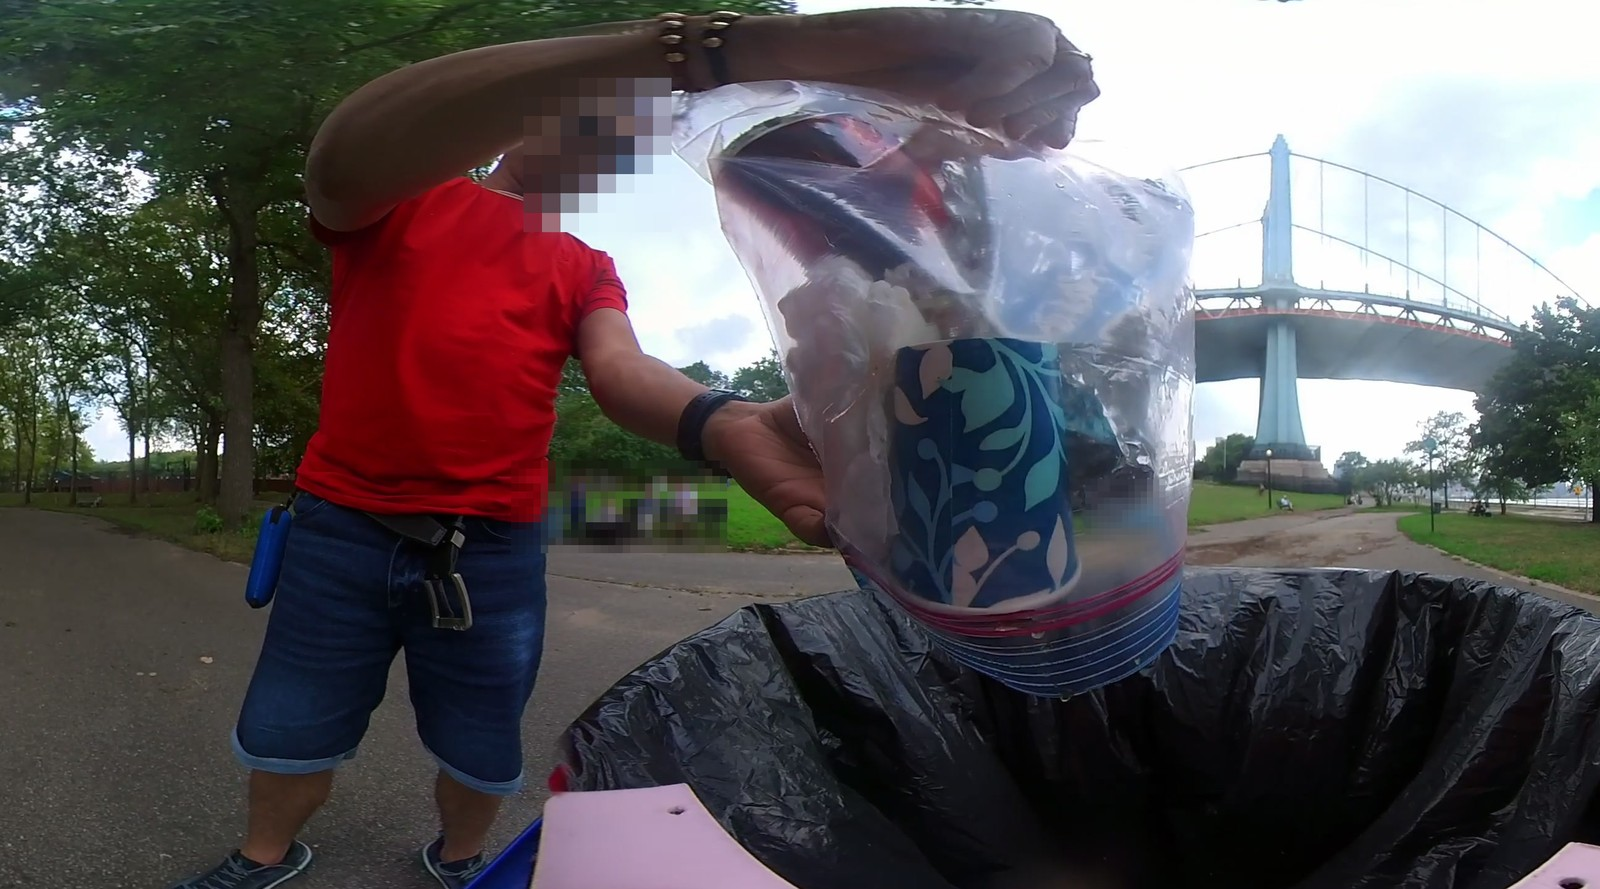
\includegraphics[width=\linewidth]{figures/vignettes/b_astoria_disposal.jpg}
    \caption{Astoria Park}
  \end{subfigure}\hfill
  \begin{subfigure}[t]{0.30\textwidth}
    \centering
    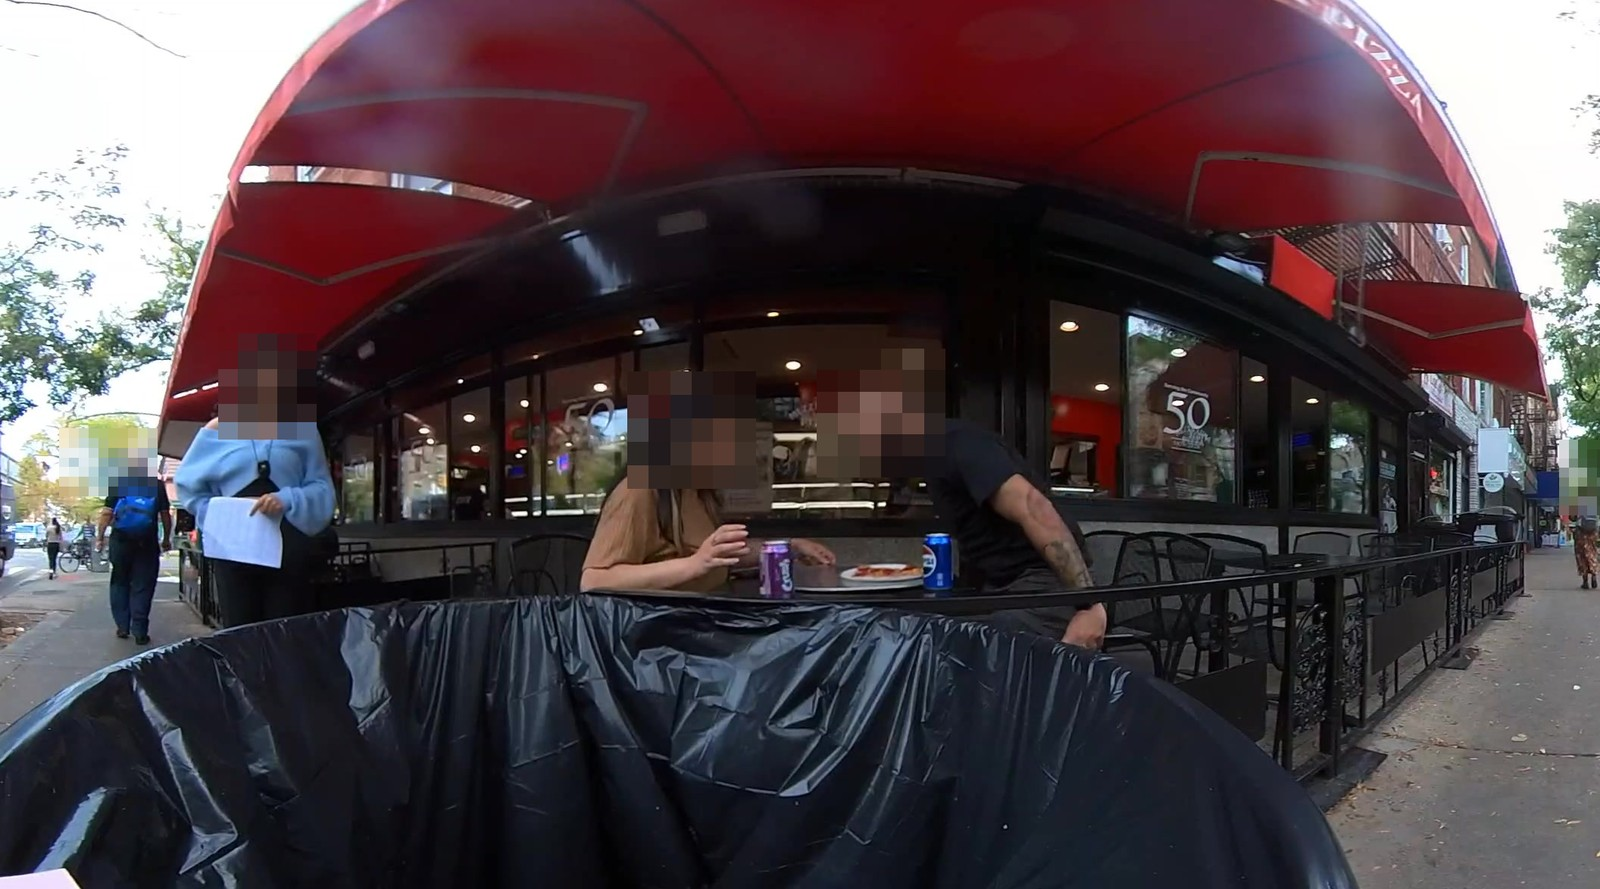
\includegraphics[width=\linewidth]{figures/vignettes/i_arthur_table.jpg}
    \caption{Little Italy}
  \end{subfigure}

  \medskip

  \begin{subfigure}[t]{0.30\textwidth}
    \centering
    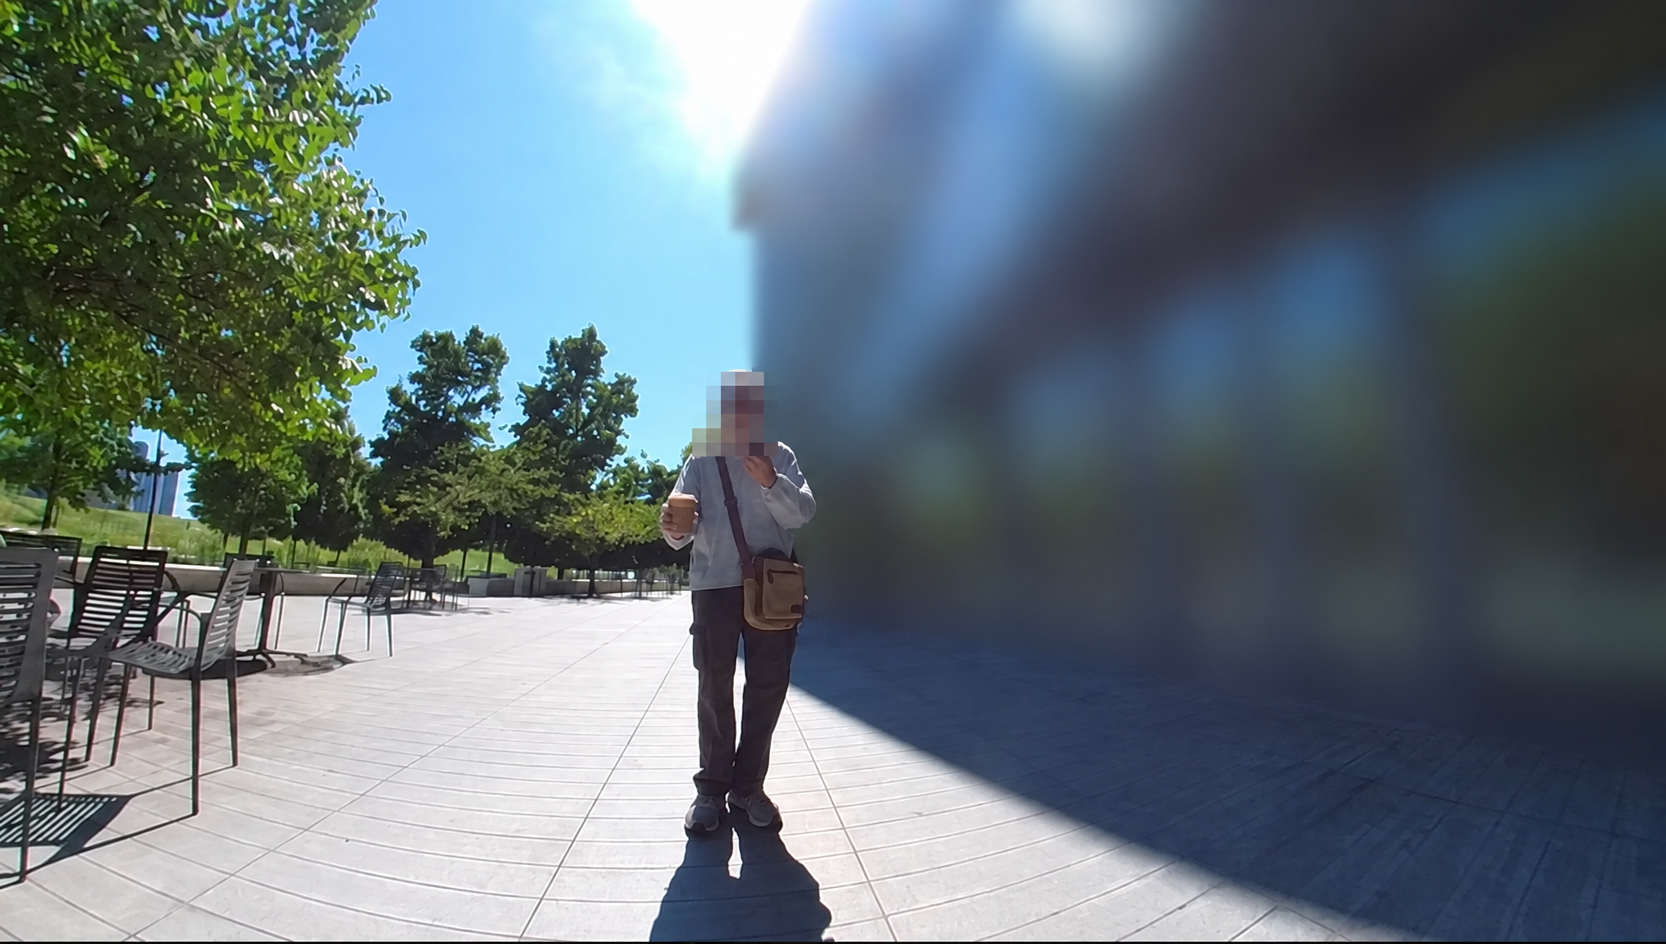
\includegraphics[width=\linewidth]{figures/vignettes/l_manhattan_cup.png}
    \caption{Campus caf\'e}
  \end{subfigure}\hspace{0.05\textwidth}
  \begin{subfigure}[t]{0.30\textwidth}
    \centering
    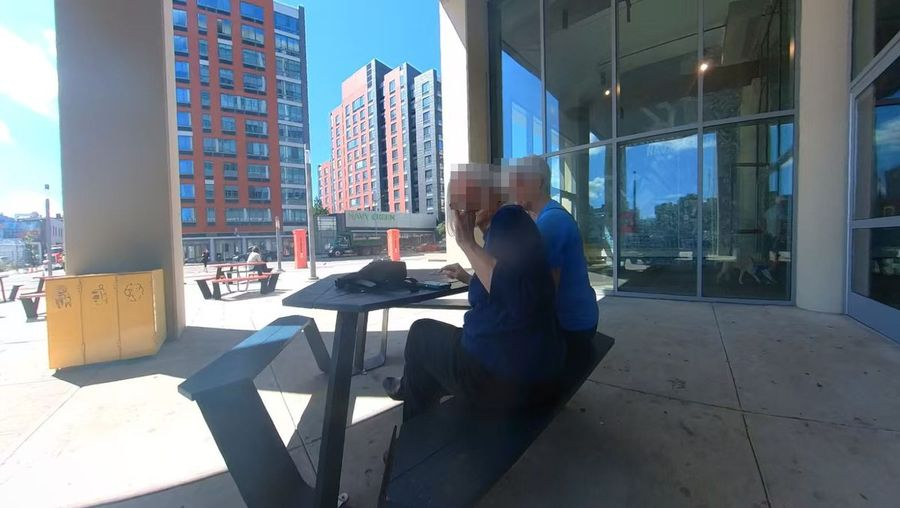
\includegraphics[width=\linewidth]{figures/vignettes/o_navyyard_wave.jpg}
    \caption{Brooklyn Navy Yard}
  \end{subfigure}

  \caption{Illustrative encounters with the Trashbot at five deployment sites, one in each New York City borough, viewed from the robot's onboard camera (faces obscured). At Tappen Park, TP-P07 reaches from a bench toward the receptacle with a bottle. At Astoria Park, AP-P02 empties a sealed bag into the receptacle. In Little Italy, the Trashbot stops beside a sidewalk table as LI-P26 reaches across its rim. At Campus Caf\'e, CC-P04 approaches while holding a coffee cup and a phone. At Navy Yard, NY-P08 gestures toward the onboard camera.}
  \Description{Five photographs from the Trashbot's onboard camera, showing encounters at one deployment site in each New York City borough. At Tappen Park, a person seated on a bench reaches toward the receptacle with a bottle. At Astoria Park, a person empties a bag into the receptacle on a park path. In Little Italy, a person seated at a sidewalk table reaches across the rim. At Campus Caf\'e, a person approaches while holding a coffee cup and a phone. At Navy Yard, a seated person gestures toward the camera. Faces are obscured.}
  \label{fig:site-encounters}
\end{figure*}

\begin{figure*}[ht]
    \centering
    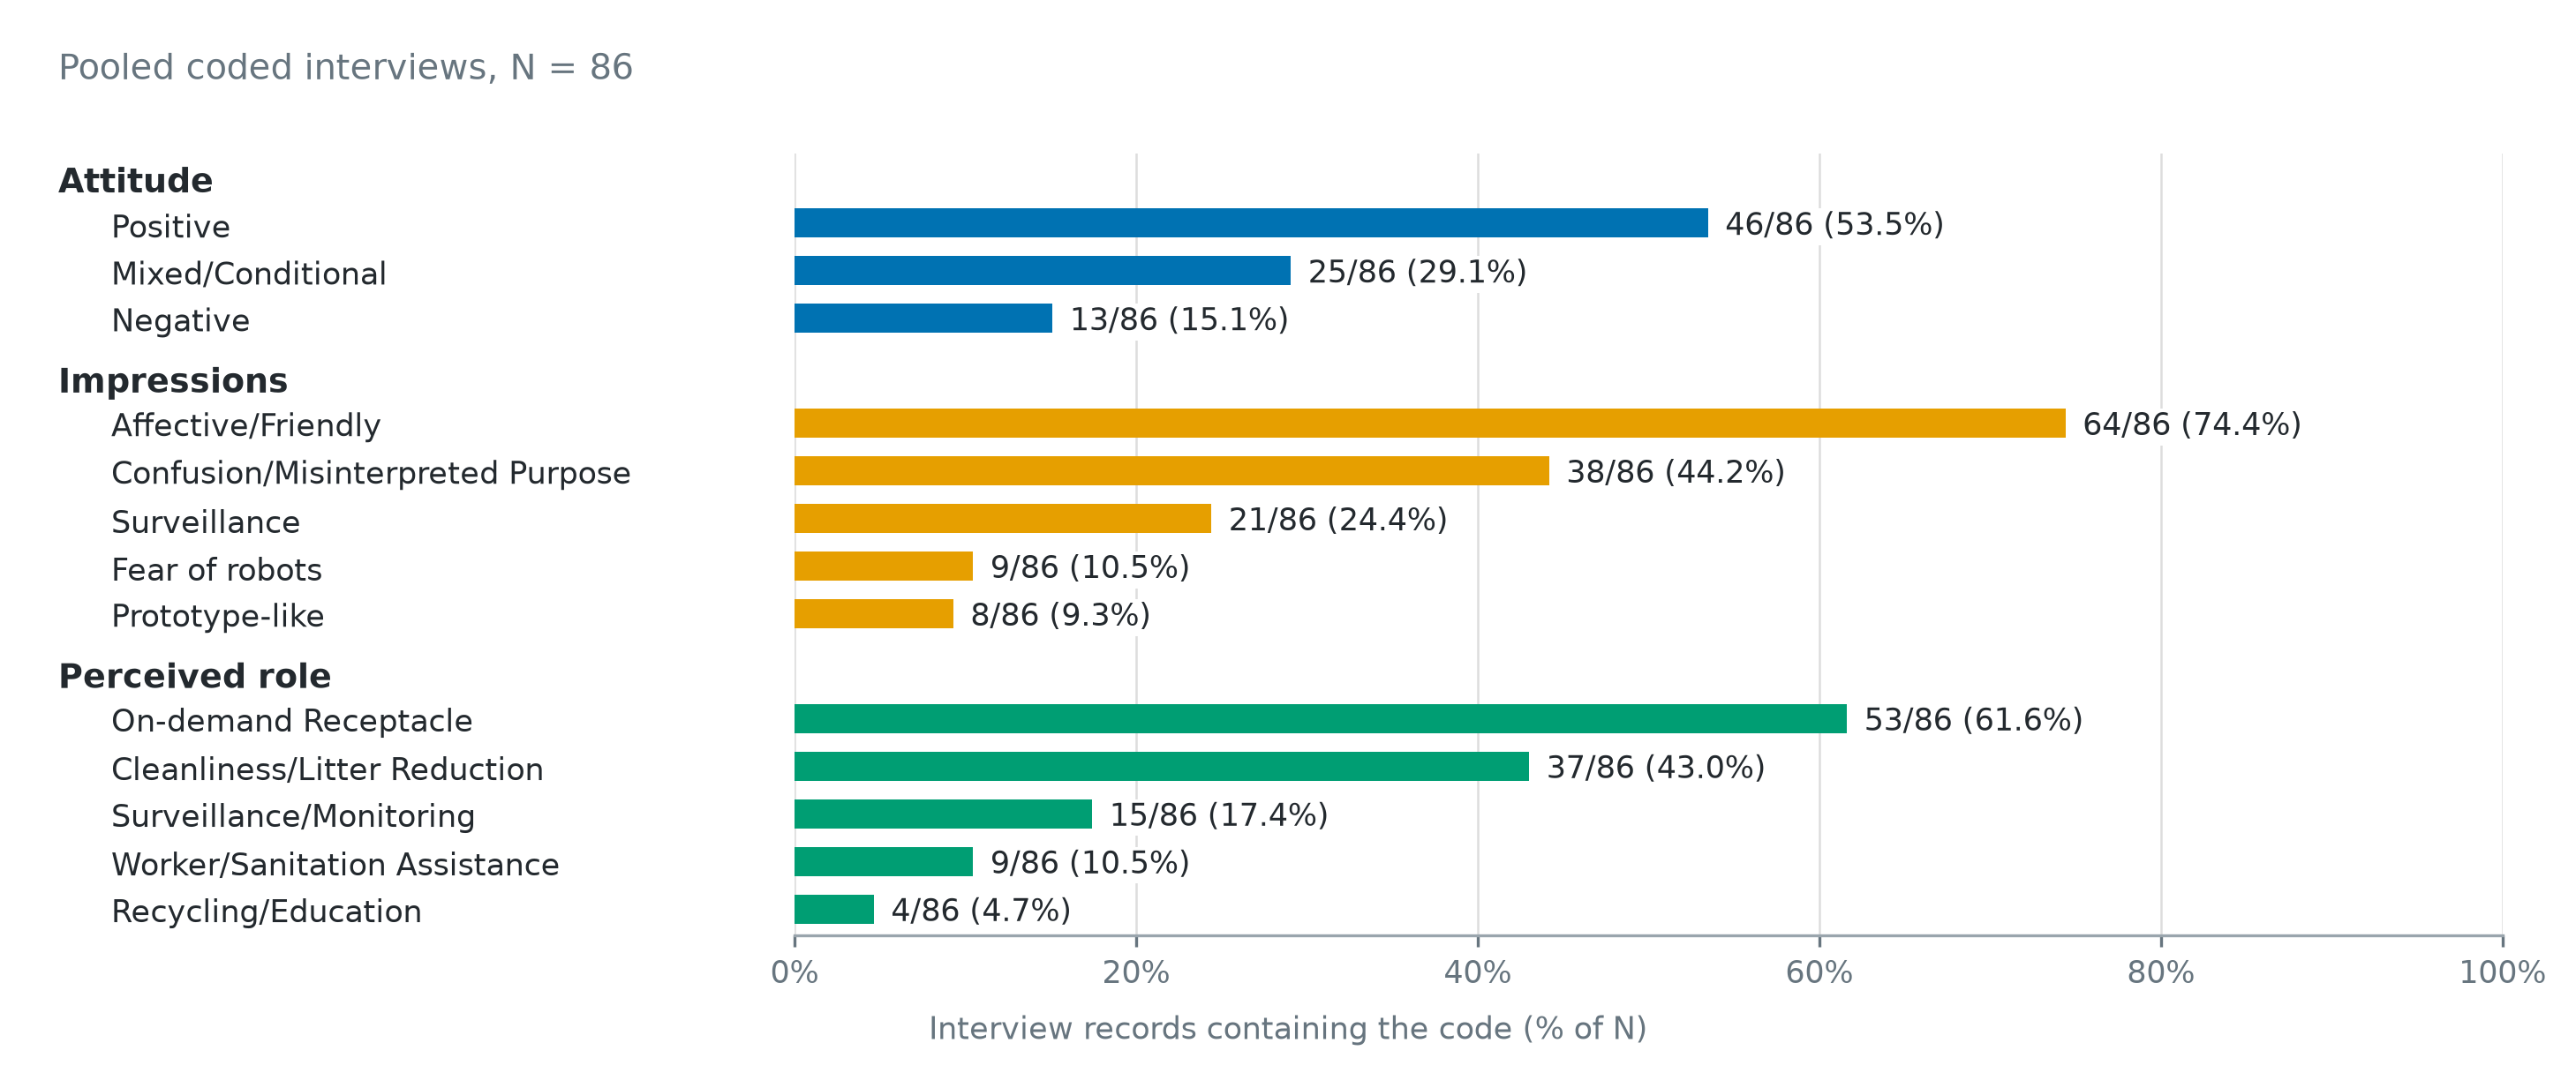
\includegraphics[width=0.95\textwidth]{figures/fig_5_1_all_sites.png}
    \caption{Prevalence of attitude, impression, and perceived-role codes across the pooled interview corpus ($N=86$ interview records). Bars show the share of records containing each code, so percentages within a group do not sum to 100\%.}
    \Description{Horizontal bar chart summarizing RQ1 interview codes across 86 records. Attitudes include 46 positive, 25 mixed or conditional, and 13 negative records. Impression codes include affective or friendly impressions in 64 records, confusion or misinterpreted purpose in 38, surveillance in 21, fear of robots in 9, and prototype-like impressions in 8. Perceived roles include on-demand trash receptacle in 53 records, cleanliness or litter reduction in 37, surveillance or monitoring in 15, worker or sanitation assistance in 9, and recycling or education in 4. Impression and perceived-role codes are nonexclusive.}
    \label{fig:rq1-pooled-codes}
\end{figure*}

\subsubsection{Attitudes}

Positive attitudes were the most frequent evaluation of the Trashbot. Forty-six of the 86 records (53.5\%) contained a positive attitude, 25 (29.1\%) contained a mixed or conditional attitude, and 13 (15.1\%) contained a negative attitude. Positive accounts commonly described the robot as useful, appealing, or appropriate for waste disposal. At the Brooklyn Navy Yard, NY-P10 called the Trashbot \emph{pretty cute} and later said, \emph{``I do like this one. I genuinely do.''}

Mixed or conditional attitudes combined approval with a condition on where or how the robot should operate. Participants raised issues such as pedestrian traffic, reliability, privacy, and the possibility of damage. AP-P04 expressed this distinction directly: \emph{``So, again, conceptually, I think it's a great idea. Practically, I think you're going to figure out where it works and where it doesn't.''} These participants often supported the service concept while reserving judgment about particular deployments.

Negative evaluations were less frequent. They included accounts that considered the robot unnecessary, unsuitable for a particular setting, or undesirable as a public technology. Attitude therefore captured participants' overall evaluation of the Trashbot, while more specific concerns about cameras, operation, or local fit were coded separately when present.

\subsubsection{Impressions}

Participants' first impressions of the Trashbot ranged from amusement and curiosity to uncertainty and concern. Affective or friendly impressions appeared in 64 of the 86 records (74.4\%), making this the most frequent impression code. Participants often described the robot as \textit{cool}, \textit{cute}, \textit{interesting}, or \textit{funny}, and some emphasized surprise at seeing a familiar object move through public space. AP-P01 recalled, \emph{``I was very curious.''} Fear of robots was much less common, appearing in 9 records (10.5\%). These reactions sometimes drew on broader concerns about autonomous systems, but they did not necessarily imply rejection of the Trashbot itself. A participant could find the encounter novel or appealing while still expressing unease about robots.

Confusion or a misinterpreted purpose appeared in 38 records (44.2\%). Participants could often identify the Trashbot as some kind of trash-related object while remaining unsure what its mobility, camera, or autonomy were meant to accomplish. In some cases, this produced an alternative interpretation altogether. AP-P13, for example, recalled, \emph{I was confused, I didn't know what it was for,''} adding that \emph{``it was like a toy.''} NY-P13 similarly suggested that \emph{``the trash can would need to be labeled.''} Prototype-like impressions, which appeared in 8 records (9.3\%), reflected a related uncertainty about the robot's status rather than its purpose: participants sometimes treated the Trashbot as an experimental object rather than a ready-to-use public service. AP-P04, for instance, assumed that \emph{``it's not the final product''} and asked whether \emph{``there's going to be more things ... added to this,''} later imagining what a more \emph{``manufactured version''} might look like. The camera introduced another interpretive possibility. Surveillance-related impressions appeared in 21 records (24.4\%), with some participants reading the robot not only as a service device but also as something that might record or monitor people. AP-P08 said that the robot \emph{``reminds me [of] robotic police,''} later connecting this impression to the camera and privacy concerns, while NY-P08 described the Trashbot as \emph{``a little startling.''} These reactions show that the robot's visible form provided an initial reference point without fully explaining either what its robotic features were for, whether it represented a finished public service, or what role its sensing might play.

\subsubsection{Perceived roles}

Participants most often understood the Trashbot in terms of what it could do for waste disposal and cleanliness, and these interpretations shaped whether the robot seemed useful. The most common role was an on-demand receptacle, appearing in 53 of 86 records (61.6\%). Here, participants understood mobility as making a trash can more accessible by bringing it closer to people. At the Brooklyn Navy Yard, NY-P11 asked whether the Trashbot was \emph{``going around so people can throw stuff in the garbage?''} and later said, \emph{``I could see it being useful.''} Cleanliness or litter reduction appeared in 37 records (43.0\%). LI-P03, for instance, said, \emph{``just to see any type of effort to clean up the streets is great, because we need that,''} noting that existing cans could be \emph{``overflowing or not available...or not maintained correctly.''} These two perceived roles often reinforced one another, since bringing a receptacle closer to users was one way participants imagined the robot contributing to cleaner public space.

Other roles focused on what the Trashbot's additional robotic features might enable beyond disposal itself. Surveillance or monitoring appeared in 15 records (17.4\%), extending the surveillance-related impressions described above. Whereas the visible camera could initially make the robot seem startling, some participants also saw it as serving a monitoring function. LI-P03, for example, described cameras as potentially useful for safety because \emph{``maybe people think twice before they come in a crime...''} The camera could therefore make the robot seem useful in an additional way. 

Worker or sanitation assistance appeared in 9 records (10.5\%). LI-P17, who identified themselves as a sanitation worker, explained, \emph{``It looks like it makes people's job [and] my job easier.''} They also weighed whether the robot might reshape sanitation work—allowing workers to focus on more demanding tasks while also raising the possibility that employers could reduce staffing. In this sense, the robot’s usefulness was judged in relation to existing labor arrangements. As we will present in Section~\ref{sec:site-sensemaking}, these judgments were also shaped by the services, staffing, and waste-management arrangements already present at particular sites. Recycling or educational roles were less frequent, appearing in 4 records (4.7\%). LI-P28 suggested that \emph{it would be really interesting to have one recycling can''} that could tell users, \emph{no, no, sorry, don't put that paper in here.''} In this account, the robot's usefulness extended beyond making disposal more accessible to helping guide how waste should be sorted. Overall, whether participants saw the Trashbot as an on-demand receptacle, a tool for reducing litter, a monitoring device, an assistant to sanitation workers, or a recycling aid, these perceived roles gave them different grounds for judging what the robot was useful for and what it added to the space during the encounter.

\subsubsection{Across sites}

Table~\ref{tab:codes-by-site-5-1} compares the RQ1 codes across the five deployment sites. Because impression and perceived-role codes could co-occur within an interview record, the table describes the prevalence of each interpretation rather than mutually exclusive groups.

\begin{table*}[t]
  \caption{Interview-code prevalence by site for RQ1. Each cell reports the number of interview records containing the code over the number of records represented at that site ($n/N$). Records may contain multiple codes or no applicable code within a category, so counts within each category need not sum to $N$. Sites: Tappen Park (TP), Astoria Park (AP), Little Italy (LI), Campus caf\'e (CC), and Brooklyn Navy Yard (NY).}
  \label{tab:codes-by-site-5-1}
  \small
  \begin{tabular}{@{}lcccccc@{}}
    \toprule
     & TP & AP & LI & CC & NY & All sites \\
     & $N=10$ & $N=13$ & $N=32$ & $N=16$ & $N=15$ & $N=86$ \\
    \midrule
    \multicolumn{7}{@{}l}{\textbf{Attitude}} \\
    \quad Positive & 7/10 & 8/13 & 14/32 & 10/16 & 7/15 & 46/86 \\
    \quad Negative & 0/10 & 1/13 & 7/32 & 2/16 & 3/15 & 13/86 \\
    \quad Mixed/Conditional & 3/10 & 3/13 & 11/32 & 4/16 & 4/15 & 25/86 \\
    \addlinespace
    \multicolumn{7}{@{}l}{\textbf{Impressions}} \\
    \quad Affective/Friendly & 7/10 & 9/13 & 27/32 & 13/16 & 8/15 & 64/86 \\
    \quad Confusion/Misinterpreted Purpose & 4/10 & 6/13 & 17/32 & 4/16 & 7/15 & 38/86 \\
    \quad Surveillance & 1/10 & 3/13 & 8/32 & 5/16 & 4/15 & 21/86 \\
    \quad Prototype-like & 0/10 & 3/13 & 2/32 & 3/16 & 0/15 & 8/86 \\
    \quad Fear of robots & 1/10 & 1/13 & 4/32 & 1/16 & 2/15 & 9/86 \\
    \addlinespace
    \multicolumn{7}{@{}l}{\textbf{Perceived role}} \\
    \quad On-demand Trash Receptacle & 5/10 & 8/13 & 18/32 & 11/16 & 11/15 & 53/86 \\
    \quad Cleanliness/Litter Reduction & 5/10 & 7/13 & 16/32 & 5/16 & 4/15 & 37/86 \\
    \quad Worker/Sanitation Assistance & 1/10 & 2/13 & 4/32 & 1/16 & 1/15 & 9/86 \\
    \quad Surveillance/Monitoring & 2/10 & 3/13 & 3/32 & 4/16 & 3/15 & 15/86 \\
    \quad Recycling/Education & 0/10 & 1/13 & 1/32 & 2/16 & 0/15 & 4/86 \\
    \bottomrule
  \end{tabular}
\end{table*}

Several patterns were shared across sites. Positive was the largest attitude category at each site, although its prevalence varied from 14 of 32 records in Little Italy to 7 of 10 at Tappen Park. Affective or friendly impressions were also the most frequent impression code at every site. The on-demand receptacle role appeared in half or more of the records at each site, with the highest proportions at the Brooklyn Navy Yard (11/15) and campus caf\'e (11/16). At Tappen Park, on-demand receptacle and cleanliness/litter reduction appeared equally often (5/10 each). These distributions indicate that participants across sites commonly recognized the Trashbot as an approachable waste-related service.

The distributions also differed in what participants found uncertain or salient. Confusion or a misinterpreted purpose appeared in 17 of 32 Little Italy records and 7 of 15 Brooklyn Navy Yard records, compared with 4 of 16 at the campus caf\'e. Surveillance impressions appeared at all five sites but were least frequent at Tappen Park (1/10). Prototype-like impressions were recorded at Astoria Park, Little Italy, and the campus caf\'e, but not at Tappen Park or the Brooklyn Navy Yard. Fear of robots remained uncommon across the corpus.

Perceived roles varied in a similar way. Cleanliness and litter reduction were especially prominent at Astoria Park (7/13), Little Italy (16/32), and Tappen Park (5/10), while fewer Brooklyn Navy Yard records assigned the Trashbot that role (4/15). Surveillance or monitoring appeared in 4 of 16 campus caf\'e records and in 3 of 15 Brooklyn Navy Yard records, compared with 3 of 32 in Little Italy. Worker assistance appeared at every site but remained uncommon, and recycling or education appeared only at Astoria Park, Little Italy, and the campus caf\'e.

The site-level comparison therefore shows a common starting point alongside different emphases. Across sites, participants often recognized a mobile waste-disposal service and responded to it positively or affectively. Their accounts differed more in what they thought the robot added to that familiar function. Some emphasized easier access to a receptacle or cleaner public space, while others attended to the camera, existing sanitation work, or uncertainty about why the trash can needed robotic capabilities. Section~\ref{sec:process} examines how participants developed these interpretations through questioning and reasoning.

\subsection{Interpreting the Trashbot: Question-driven and Reasoning-based Sensemaking} 
\label{sec:process}

We examined the interpretive strategies participants used to make the Trashbot’s presence intelligible in addressing \textbf{RQ2}. Among the strategies identified in our analysis, we focus here two broad forms that recurred across the data: \textit{question-driven sensemaking} and \textit{reasoning-based sensemaking}. Question-driven accounts surfaced uncertainty through WHAT, HOW, and WHO questions about the robot’s purpose, operation, and the actors behind it. Reasoning-based accounts instead worked through ambiguity by drawing inferences, projecting possible actions and consequences, and making analogies from available cues. Figure~\ref{fig:sensemaking-all-sites}a visualizes the percentage of interview records containing each interpretive-strategy code reported here.

\subsubsection{WHAT: identifying the robot and its role}
WHAT questions were raised by 33 participants (38.4\%), making them the most common question type. For some, these questions surfaced immediately; NY-P13 described \emph{``what does it do?''} as \emph{the first question.} These questions concerned identifying the Trashbot's function and role in the space. Typical WHAT questions included:

\begin{itemize}
    \item \emph{``What is this/What does it do?''} (\textit{e.g.}, AP-P04, LI-P22, NY-P10)
    \item \emph{``What is the point or purpose of it?''} (\textit{e.g.}, AP-P06, LI-P18, LI-P21)
    \item \emph{``What is the camera or collected data for?''} (\textit{e.g.}, LI-P01, TP-P04, NY-P15)
\end{itemize}

Some participants phrased similar uncertainties as WHY questions, such as \emph{``why a trash can needed to move?''}. We grouped these with WHAT questions because they likewise concerned the purpose of its robotic features. Participants were often able to recognize the Trashbot as a trash can, but were less certain about what made it a \emph{robotic} trash can or why such a device was needed in the space. In this sense, the Trashbot was only partially legible. LI-P18, for example, asked \emph{``what is the purpose of that exactly?''}, expressing uncertainty about the function of the robot's mobility. The camera could further complicate this interpretation: LI-P07 initially thought it was there to make sure ``nobody was throwing their garbage'' into the bins, concluding that \emph{``it's not clear what it's for.''} 

WHAT questions therefore helped participants reconcile the Trashbot's familiar trash-can form with its unfamiliar robotic features by determining what those features were for. LI-P10 initially asked, \emph{``So what is it gonna do? ... It's just gonna travel around the blocks?''} After learning that the trash can's design included approaching individuals who were holding trash, they responded, \emph{``that's a good idea''} and \emph{``it's very convenient.''} NY-P08 similarly emphasized that the robot's purpose needed to be explicit: after saying they had ``no idea what it's trying to do,'' they explained that public robots made more sense when their purpose was ``made clear,'' for example by communicating that they were there to collect trash. Thus, having answers to WHAT questions did more than identify the object: it connected the robot's movement and sensing capabilities to an intended service, enabling participants to judge whether that service was useful and made sense.

\subsubsection{HOW: understanding operation and interaction}
HOW questions were raised by 30 participants (34.9\%). These questions concerned how the Trashbot worked and, correspondingly, how people were expected to interact with it. Rather than asking what service the robot provided, participants were curious to know the relationship between its sensing and movement and their own actions. Typical HOW questions included:
\begin{itemize}
    \item \emph{``How does it work?''} (\textit{e.g.}, LI-P03, LI-P10, LI-P16)
    \item \emph{``How do you control it/is it autonomous?''} (\textit{e.g.}, LI-P01, LI-P11)
    \item \emph{``How do I make it approach me?''} (\textit{e.g.}, CC-P01, NY-P12, NY-P13)
\end{itemize}

Participants' HOW questions first concerned the robot's operation: what made it move, what its camera sensed, and whether its behavior was autonomous or controlled by someone else. LI-P10, for example, asked, \emph{``How does it work? Well, it's battery-operated or something?''}, while LI-P01 asked directly, \emph{``do you control them?''} Participants also tried to infer how sensing produced movement. LI-P16 asked whether the robot was \emph{``supposed to move when [it] sees people''} or instead \emph{``approach to people to dump the garbage.''} At the campus café, participants offered competing explanations of the camera's role: one thought it turned to \emph{``see where the trash is,''} while another thought it was \emph{``looking at the people to see if they have trash to throw away.''} These questions sought to establish the mechanism behind the robot's apparently autonomous behavior: what it detected and how that detection translated into action. 

A related set of HOW questions also concerned how people were supposed to interact in that operation. Knowing that the Trashbot could approach people did not necessarily explain who should initiate the encounter or what action would summon it. NY-P12, for example, asked whether \emph{``the trash can [would] follow, go near people''} who had trash, while CC-P01 tried waving but remained \emph{``confused how to make it approach to me,''} explaining, \emph{``I don't know if it attracted to my move or if it approached to me by itself.''} LI-P07 similarly wondered \emph{``how the people know''} they were allowed to use it and \emph{``how they interact with it.''} Thus, HOW questions addressed both sides of the encounter: how the robot produced its behavior and how a person's actions were expected to produce a response from it.

\subsubsection{WHO: attributing stakeholders and responsibility}
WHO questions were raised by 14 participants (16.3\%), occurring less frequently than WHAT and HOW. These questions concerned the people or institutions behind the Trashbot: who created or deployed it, who was monitoring it, and who could access the information it collected. Unlike HOW questions about the mechanisms producing the robot's behavior, WHO questions sought to locate those mechanisms within a person or institutional arrangement. Typical WHO questions included:

\begin{itemize}
    \item \emph{``Who is watching behind the scene?''} (\textit{e.g.}, AP-P01)
    \item \emph{``Who made it/is it an official thing?''} (\textit{e.g.}, LI-P02, LI-P33, TP-P04)
    \item \emph{``Who can access [the data]?''} (\textit{e.g.}, NY-P12, CC-P13)
\end{itemize}

Participants first sought to identify who had placed the robot in the space and on whose behalf it was operating. TP-P04, for example, initially assumed that the Trashbot \emph{``belonged to, like, the sanitation department, or parks department,''} but the camera made that attribution less certain: \emph{``you don't know who it is, somebody might be doing surveillance.''} LI-P02 similarly said that, despite finding the robot interesting, they \emph{``can't figure out who made it or, like, if it's an official thing.''} For this participant, identifying the actor behind the robot was itself important to understanding the encounter: \emph{``who you are and what you're doing is important,''} because people needed to know \emph{``where you're coming from, not just anybody.''} WHO questions therefore situated the robot within a recognizable institutional relationship, distinguishing, for example, a sanitation service or university research project from an unidentified actor operating equipment in public space.

Questions about who was behind Trashbot became especially consequential around its camera and data practices. AP-P01 wondered \emph{who is watching behind the scene?''} and initially assumed \emph{the city has, like, cameras on this,''} while NY-P12 described their privacy concern as \emph{``what's it filming and how's it being used and who can access that.''} These accounts show that participants wanted to know not only what the robot collected, but who received that information and was responsible for its use. Resolving WHO questions therefore gave participants a basis for judging the legitimacy of its presence, the appropriateness of its sensing practices, and who could be held accountable for them.

\subsubsection{Reasoning-based Sensemaking Strategies} 
Question-driven sensemaking made participants' uncertainties explicit, but participants did not always respond to ambiguity by asking for an answer. They also constructed provisional interpretations from information already available to them. We observed the follwing three recurring forms of this reasoning. These strategies were not mutually exclusive. Participants often combined them as they worked from an initially ambiguous encounter toward an interpretation of what the Trashbot was doing, how it might behave, and what its presence could mean.

\paragraph{Inferring from Appearance and Behavior}
Participants often inferred the Trashbot's purpose and operation from features they could directly observe, including its trash-can form, movement, camera, and responses to people. CC-P04, for example, initially thought it was \emph{``just rolling,''} but after noticing that it \emph{``stopped if it saw a person''} and that \emph{``the camera looked at the person,''} concluded that it was responding to people and approached it with an empty coffee cup. AP-P04 combined its Roomba-like body with the visible garbage cans to guess that \emph{``maybe this is for trash pickup.''} In this way, participants treated the robot's appearance and behavior as evidence from which to construct possible explanations of what it was doing and how it worked.

\paragraph{Projecting Plausible Scenarios}
Participants also reasoned by imagining situations that extended beyond what they directly observed. These projections helped them anticipate how the Trashbot might behave or what consequences its deployment could produce. For example, NY-P13 imagined the robot mistakenly entering a bike path after interpreting someone's wave as a command, while LI-P17 considered both the possibility that automation could reduce sanitation jobs and that it could instead make those jobs easier. For AP-P01, they anticipated that people might \emph{``mess''} with or \emph{``hit''} the robots. Such scenarios allowed participants to evaluate potential safety, labor, and social consequences before those outcomes had actually occurred.

\paragraph{Drawing on familiar comparisons}
Participants also interpreted the Trashbot by comparing it with things they were already familiar with. CC-P01 connected it to a restaurant service robot that delivered drinks, while LI-P21 compared it to autonomous wheelchairs used in airports, asking whether it relied on \emph{the same technology} as wheelchairs that \emph{don't need a pusher.} These familiar systems provided reference points for understanding the Trashbot's mobility and service role. Comparisons could also carry expectations about risk: AP-P08 drew on Citi Bike and Lime Bike rollouts to anticipate vandalism and eventual normalization, while LI-P18 connected its apparently self-directed movement to narratives about robots having \emph{a mind of its own.} These comparisons therefore helped participants interpret not only what the Trashbot might do, but also whether it seemed trustworthy or legitimate.


\subsection{Situating the Trashbot: Local Knowledge and Personal Experience}
\label{sec:site-sensemaking}

\begin{figure*}[ht]
  \centering
  \begin{subfigure}[t]{0.52\textwidth}
    \centering
    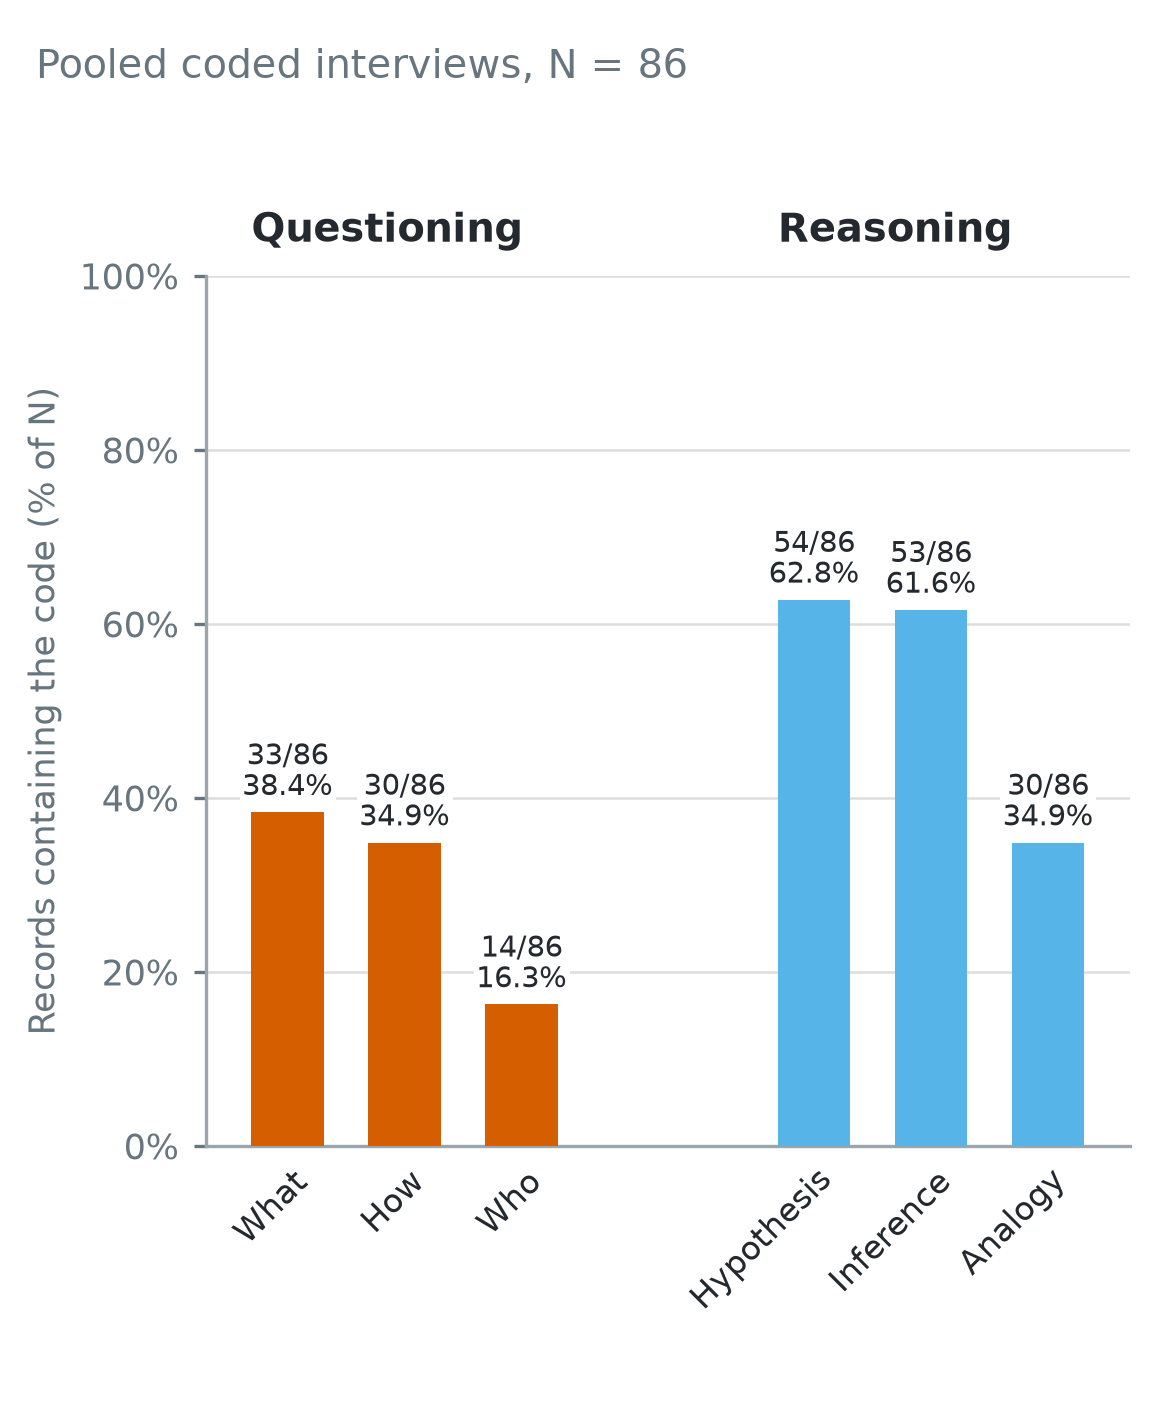
\includegraphics[width=\linewidth]{figures/fig_5_2_all_sites.png}
    \caption{Sensemaking strategies}
    \label{fig:strategies}
  \end{subfigure}
  \hfill
  \begin{subfigure}[t]{0.415\textwidth}
    \centering
    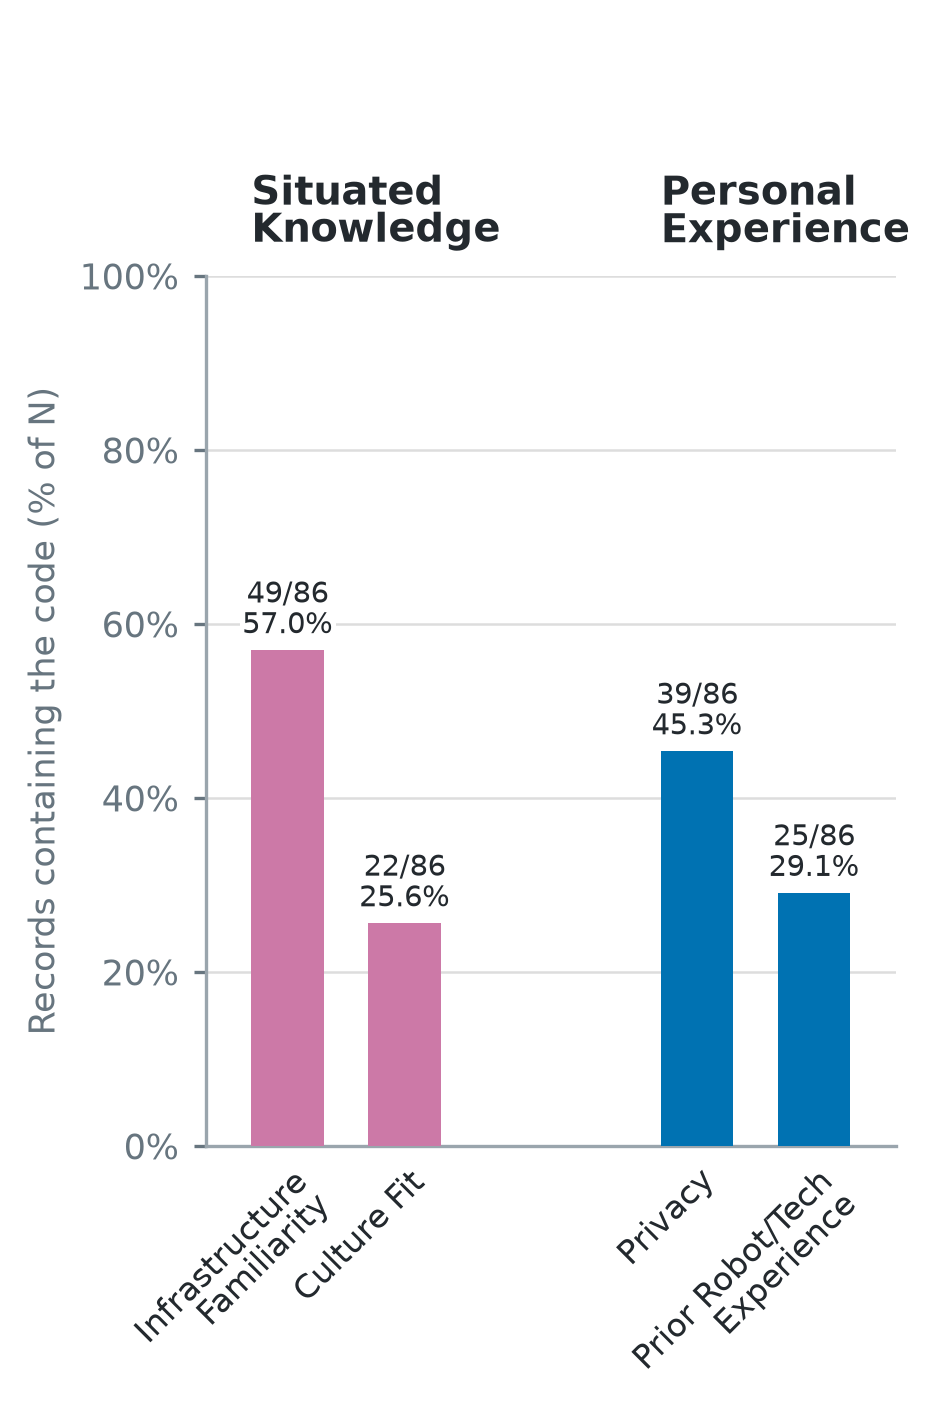
\includegraphics[width=\linewidth]{figures/fig_5_3_all_sites.png}
    \caption{Knowledge resources}
    \label{fig:resources}
  \end{subfigure}
  \caption{Prevalence of sensemaking codes across the pooled interview corpus ($N = 86$ interview records). (a)~Question-driven strategies (WHAT, HOW, WHO) and reasoning-based strategies (hypothesis, inference, analogy). (b)~Situated knowledge (infrastructure and familiarity, culture fit) and personal experience (privacy, prior robot or technology experience) that participants drew on. Bars show the share of records containing each code; codes are nonexclusive.}
  \Description{Two bar charts. Left chart, sensemaking strategies: What 38.4\%, How 34.9\%, Who 16.3\%; Hypothesis 62.8\%, Inference 61.6\%, Analogy 34.9\%. Right chart, knowledge resources: Infrastructure or familiarity 57.0\%, Culture fit 25.6\%; Privacy 45.3\%, Prior robot or technology experience 29.1\%.}
  \label{fig:sensemaking-all-sites}
\end{figure*}

To address \textbf{RQ3}, we examined the resources participants drew on when developing the interpretations described in Section~\ref{sec:process}. Similar forms of questioning and reasoning recurred across deployment sites, but the resources used to work through them varied. Some participants drew on knowledge of the setting itself, including existing infrastructure, familiarity with the community, and expectations about local behavior. Others relied on prior experience withrobots and related technologies and their expectation about the degree of privacy afforded by the site.  Among the resources identified in our analysis, we focus here on two broad families that were particularly relevant to the cross-site comparison: \emph{situated knowledge} and \emph{personal experience}. Situated knowledge was reflected through infrastructure or community familiarity and culture fit. Personal experience appeared through privacy and prior robot or technology experience. Figure~\ref{fig:sensemaking-all-sites}b visualizes the prevalence of the resource codes reported in this section.

\subsubsection{Situated Knowledge}
Situated knowledge concerned what participants knew about the deployment setting and how they used that knowledge to interpret the Trashbot. This included both the material and service conditions of the site and participants' understanding of its social and cultural context. Participants drew on existing infrastructure and services when judging whether the robot addressed a local need or duplicated what was already available. They also drew on familiarity with the community, including its history and expectations about how people at the site might respond to the robot.

\paragraph{Existing Infrastructure and Community Familiarity}
In 49 of 86 records (57.0\%), participants drew on infrastructure and community familiarity when interpreting the Trashbot. Participants frequently evaluated the Trashbot by comparing its proposed service with the sanitation resources already available around them. At Astoria Park, AP-09 welcomed the Trashbot because they think it is hard to find a nearby trash barrel: \emph{I do love the idea of them just roaming around...oftentimes you can't find a trash can.} LI-P03 made a similar judgment from the condition of existing infrastructure, noting that \emph{``a lot of the cans are overflowing or not available or not maintained correctly''} and therefore saw a technology intended to improve cleanliness as worthwhile. In these accounts, the Trashbot’s mobility made sense because it addressed a recognizable gap in the site’s existing sanitation services. Yet participants at the same site could read those services differently. LI-P22 saw little need for the Trashbot in Little Italy because \emph{``the community already have their cleaners and, you know, already have their porters that clean here every single day.''} Local infrastructure therefore shaped how participants judged the Trashbot’s usefulness, though not always in the same way. Participants also drew on their knowledge of this community history toward the interpretation of the Trashbot at the site. TP-P05 expressed that \emph{``it is not the ideal site''} by explaining that \emph{``you ain't in the safest park right now. This is [known as] drug city historically...you're going to get robbed by somebody around here''}. What counted as a suitable deployment site was thus anchored in participants’ understanding of the site as an existing social environment.

%might fit here instead: Similarly, LI-P17 \emph{there's a lot of, like, crackheads \ldots\ they like to knock stuff down \ldots\ Personally, over here, if it's more safer, it's more like being visualized, watched, here is perfect. Over there, it should be bad}.

\paragraph{Culture Fit}
In 22 of 86 records (25.6\%), participants used expectations about local norms, values, and behavior to judge whether the Trashbot fits that specific context. Whereas community familiarity concerned what participants knew about how a particular place functioned, culture fit concerned whether they saw the robot as compatible with how people there were expected to behave and with what the community appeared to value. AP-P04, for example, anticipated that \emph{``people don't respect [the robot]...you would probably have a much more effective deployment either in a wealthy community or [somewhere] outside of this region''}. Here, the concern was not simply knowledge of local conditions, but whether an unattended public robot would be treated in ways that allowed the service to work as intended. Culture fit could also be positive. CC-P11 saw the Trashbot as a visible sign that the site was \emph{``doing an active effort to keep it nice, the way I expect it to be,''} interpreting the robot as consistent with the environmental standards they associated with the place. LI-P21, by contrast, described the community they originally from as \emph{``very conscious about the environment''} and already relatively free of litter, making the Trashbot seem less necessary there. Their reference to the community culture assisted them to understand if the Trashbot was an appropriate addition to the site.

\subsubsection{Personal Experience}
Alongside with situated knowledge was anchored in the deployment setting, personal experience provided another source for interpreting the Trashbot. The two often worked together, as participants interpreted what they encountered through expectations and experiences formed elsewhere. These included prior experiences with cameras and surveillance, expectations about privacy, previous encounters with robots or related technologies, and familiar representations of robots. Because these experiences varied across individuals, participants at the same deployment site could interpret the same feature differently.

\paragraph{Privacy}
Participants (39/86, 45.3\%) used their understanding of privacy to judge the appropriateness of the Trashbot. Participants showed a variety of attitude towards the robot because of different attitude toward the privacy. For example, AP-P01 initially found the robot amusing but became more uneasy after noticing the camera, explaining \emph{``maybe it's a little invasive of privacy.''} CC-P16 shared a similar concern: \emph{``there is always the issue of privacy, right?...it's still not that nice to know that you are being constantly recorded''}. Other participants were less concerned about the privacy issue because they saw surveillance as already everywhere. CC-P06, for instance, said \emph{``I'm already pretty used to...phone tracking our activity across the apps, [and] being under surveillance all the time.''} Some participants also drew boundaries around where recording felt acceptable. CC-P05 distinguished public space from more private settings, saying they would object at \emph{``my workplace, or like my house, or my children's school''} but that \emph{``in the public place...I don't mind.''} These responses suggest that participants’ expectations about where and when surveillance was acceptable shaped whether the Trashbot’s camera, and by extension the robot itself, felt appropriate in the setting.

\paragraph{Prior Experience to Technology and Robots}
Participants also relyed on prior experience with robot to make sense of the Trashbot (25/86, 29.1\%). For some, this experience provided background knowledge for evaluating how the Trashbot should behave. LI-P33, who worked with robot in seminconductor manufacturing, focused on the robot's movement, suggesting that whether it would work depended on the \emph{``smoothness of the robot''} and noting that jerky motion could leave people unsure whether it was approaching them. Others compared the Trashbot with autonomous systems they already knew to anticipate possible interaction and problems. CC-P08 related to delivery robots, noting that \emph{``everyone wants to interact with it,''} while LI-P14 recalled encountering a robot dog in West Village,using that experience to interpret the Trashbot's novelty and the reactions it attracted from passersby. Participants also drew on familiar representations of robots in literature or science fiction movie to interpret the robot. For example, TP-P05 said the Trashbot \emph{``reminds me of the Jetsons. The Jetsons had a garbage can like [this],''} and AP-P04 described it as having \emph{``a mind of its own...[like] the T-1000...I do think that this is the future}. TP-P05 also invoked \emph{Judgment Day} and \emph{Skynet} when expressing distrust of technology. These prior encounters and references supplied expectations for how a robot might move, interact, or develop beyond what participants could observe from the Trashbot itself.